\part{引言}

DNS \emph{(Domain Name System)}也即域名系统,是当今互联网中不可或缺、随处可见、无比重要的一部分。DNS本质上是一个分布式数据库,能够响应互联网上用户的查找请求,将域名转换为相应的IP地址。域名作为一种方便记忆的标识名称,免去了互联网用户记忆IP地址的不便,大大简便了对互联网资源的访问,使互联网蓬勃发展,渗透入个人日常生活的所有角落成为可能。而DNS服务器 \emph{(DNS Server)} 作为DNS组成节点,让DNS这一纵贯世界、庞大而至关重要的系统运作起来,是互联网体系中不起眼却关键的组成元件。

\begin{figure}[h]
  \centering
  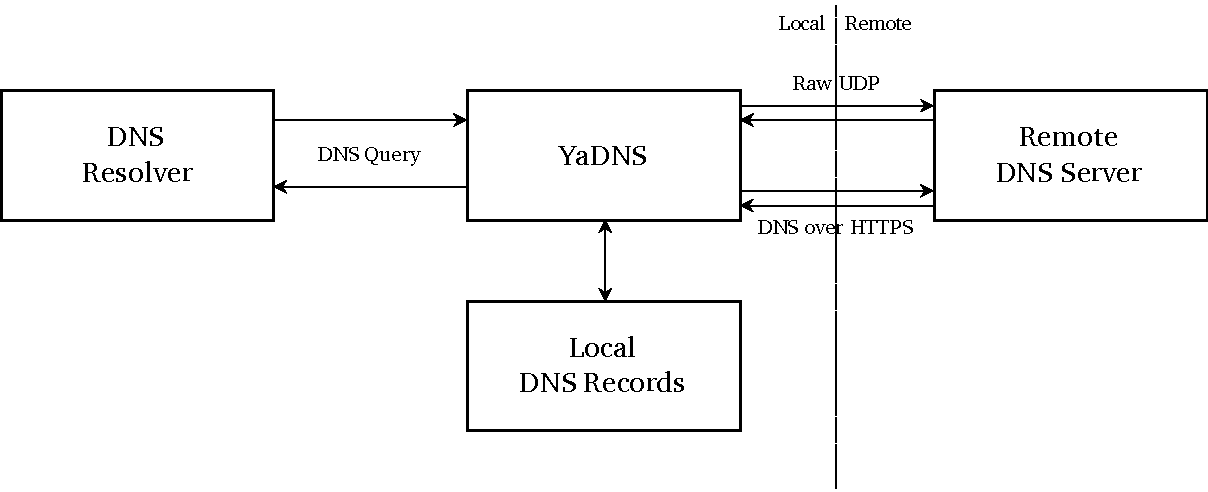
\includegraphics[width=0.85\textwidth]{figures/overview}
  \caption{YaDNS概览}
  \label{fig:overview}
\end{figure}

在本次课程设计中,我设计并实现了一个简单、高效的支持DoH \emph{(DNS over HTTPS)} 的DNS中转服务器YaDNS。YaDNS能够在53端口监听DNS查询请求,并转发到远程服务器,实现DNS代理功能。同时,YaDNS也能够加载域名记录文件,若请求命中了加载的域名记录,则直接返回,借此可以实现对DNS污染的反制、去除广告、防御恶意网址等功能。

YaDNS实现了两种对DNS请求的转发方式:普通UDP转发与DoH转发。(a) 普通的UDP转发将收到的DNS请求转发到指定远端服务器的53端口上,并将收到的应答返回给用户。YaDNS使用同一个UDP套接字 \emph{(UDP Socket)} 对所有的UDP请求进行转发,并通过对DNS消息标识符的处理来避免重复与混淆。 (b) DoH转发将DNS请求包装在一个HTTPS请求中,通过TLS连接,发送给远端DNS服务器的443端口。通过将DNS请求包装在HTTPS请求中,DoH具有更高的安全性。DNS信息不会被中间人篡改,其他人也无法收集分析用户的域名查询行为。若开启DoH转发模式,则YaDNS称为一个安全的DNS代理,修改本地DNS解析器的默认地址为YaDNS地址(也即本机),则可以将不安全的UDP查询封装为安全的DoH请求,几乎杜绝了中间人修改、查看的可能。

YaDNS实现了一个基于 \lstinline{Trie} 树的响应缓存 \emph{(Response Cache)},对于响应中的 \textbf{A类} 资源,将会缓存其中的域名与IP地址信息。缓存的生存时间由报文中资源的TTL决定。

YaDNS使用高效的数据结构存储本地加载的域名记录。YaDNS实现了一个树来存储记录,同时也实现了一个简单而小型的LRU缓存 \emph{(LRU Cache)}与自实现的域名Hash算法。对于经常访问的热点数据,能够大大提高返回速度。

项目中,我使用了成熟高效的构建工具与开发环境提高了开发效率,也利用\texttt{cmocka}测试库为对YaDNS的核心算法逻辑编写单元测试。